\subsection{Core Figures}
\begin{figure}[t]
\centering
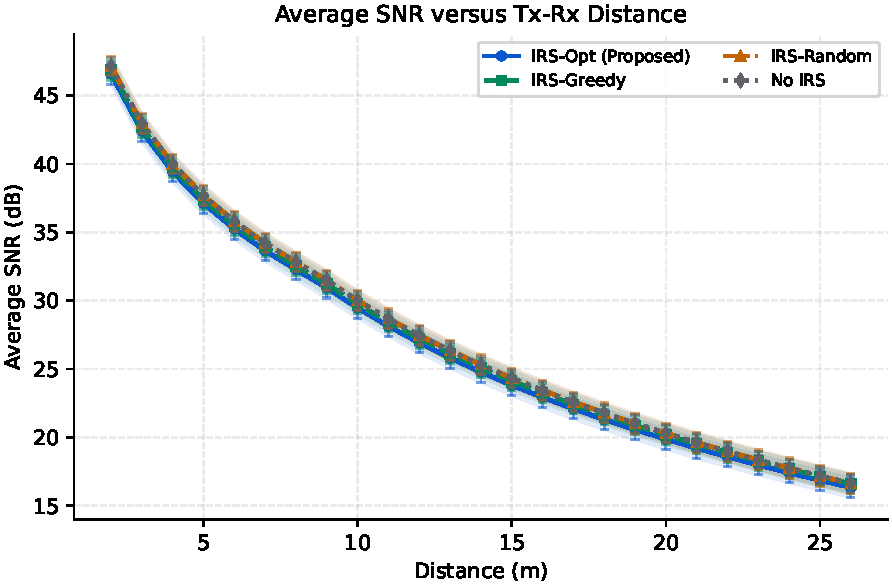
\includegraphics[width=0.95\columnwidth]{figures/generated/figure_01_snr_vs_distance.pdf}
\caption{Average SNR versus distance with confidence intervals; marker locations correspond to evaluated operating points rather than interpolated traces.}
\label{fig:figure_01_snr_vs_distance}
\end{figure}

\begin{figure}[t]
\centering
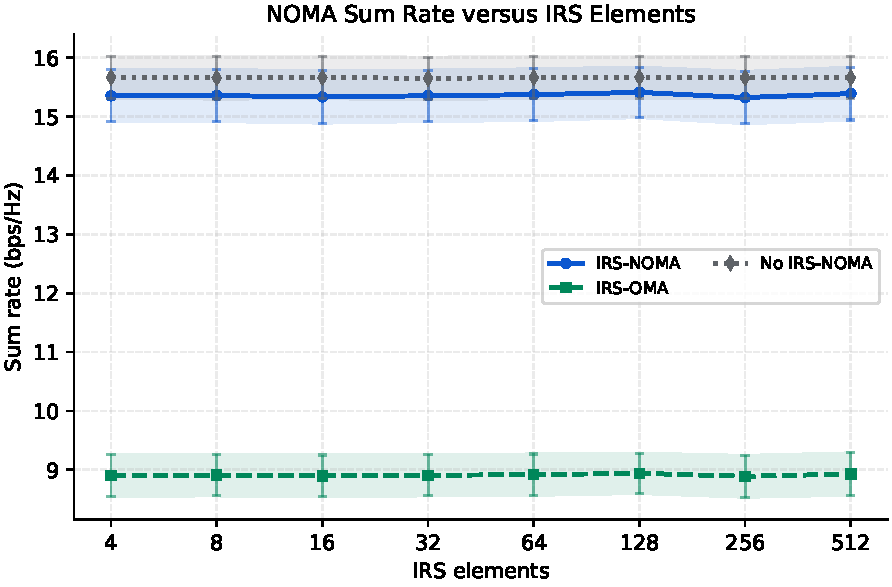
\includegraphics[width=0.95\columnwidth]{figures/generated/figure_04_noma_vs_n.pdf}
\caption{NOMA sum-rate scaling with IRS size; the proposed method tracks the highest robust joint utility as the aperture grows.}
\label{fig:figure_04_noma_vs_n}
\end{figure}

\begin{figure}[t]
\centering
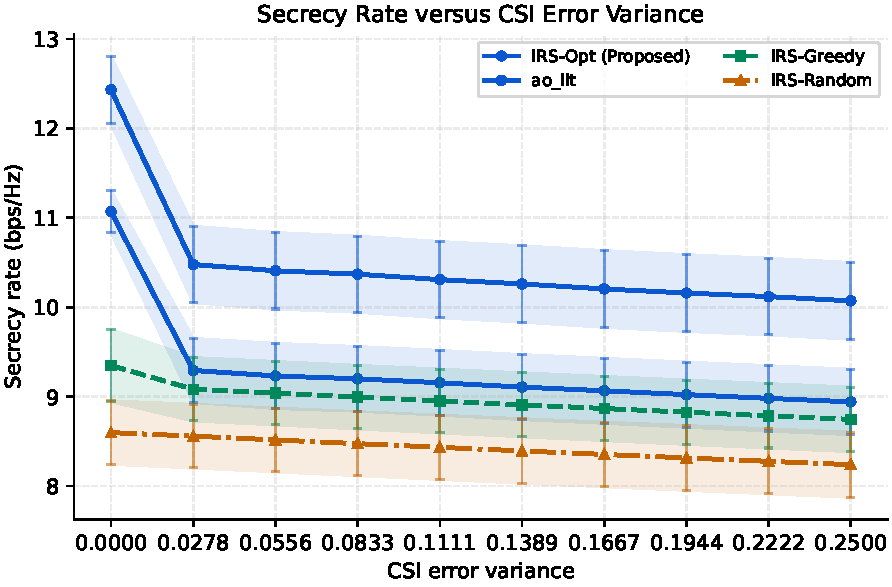
\includegraphics[width=0.95\columnwidth]{figures/generated/figure_08_secrecy_vs_csi.pdf}
\caption{Secrecy-rate robustness under CSI uncertainty, including the literature-inspired AO baseline.}
\label{fig:figure_08_secrecy_vs_csi}
\end{figure}

\begin{figure}[t]
\centering
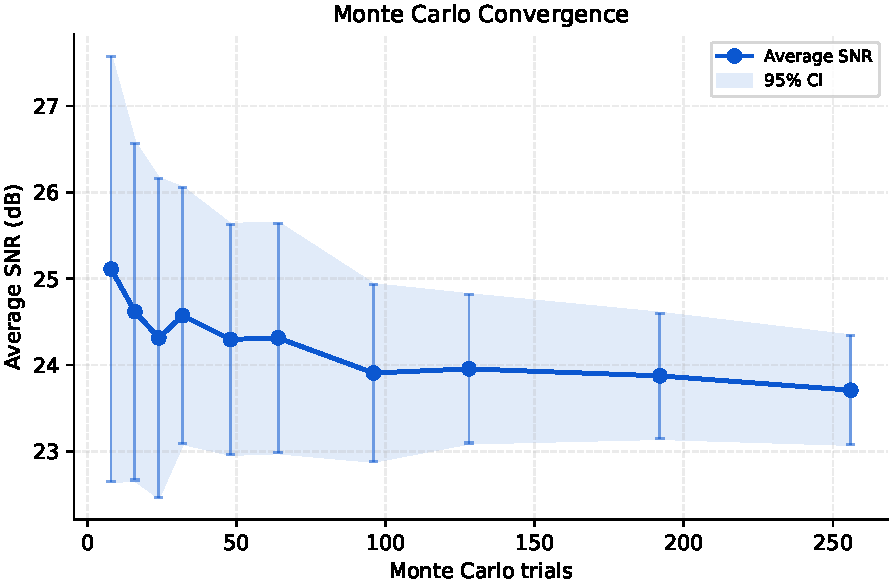
\includegraphics[width=0.95\columnwidth]{figures/generated/figure_11_convergence.pdf}
\caption{Monte Carlo convergence of the proposed solver; shrinking confidence bars indicate stabilization of the reported average SNR.}
\label{fig:figure_11_convergence}
\end{figure}

\begin{figure}[t]
\centering
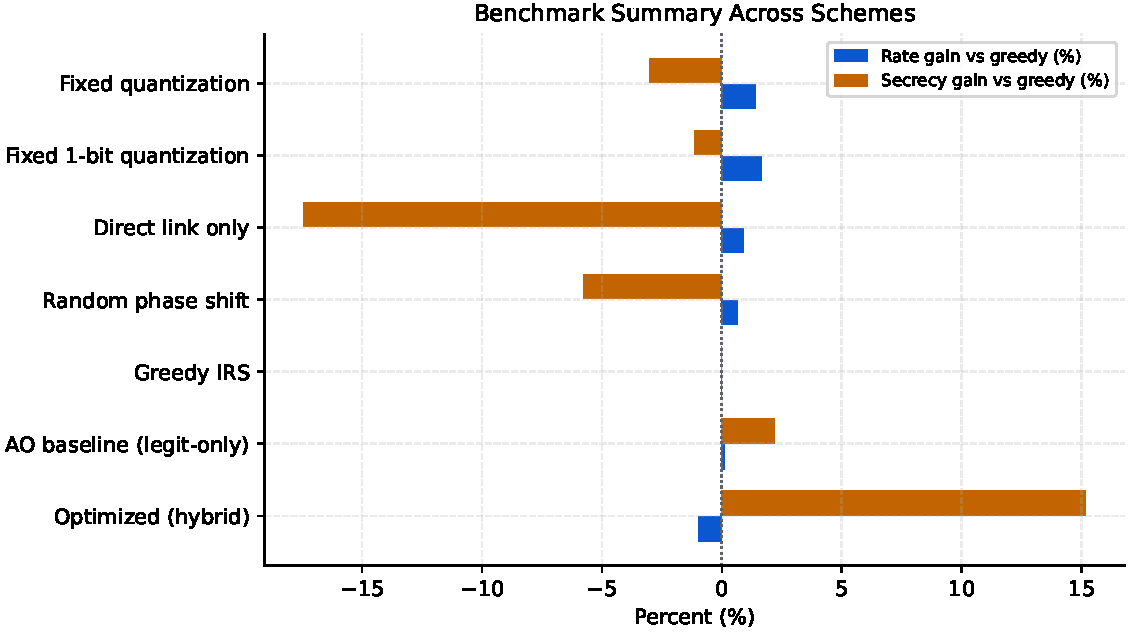
\includegraphics[width=0.95\columnwidth]{figures/generated/figure_12_comparison.pdf}
\caption{Scheme-level gains relative to greedy alignment, separating nominal-rate and secrecy improvements.}
\label{fig:figure_12_comparison}
\end{figure}
